% Build from the repository root:
% pdflatex -interaction=nonstopmode -halt-on-error -output-directory=output/pdf output/pdf/trust-me-bro-report.tex
% Implementation reviewed at 32493c2fdebcb0863e2d15ae832abedd2a55f672
% on origin/aj-arts-meta-agent-integration-fixes.
% Model observations are the author's qualitative account, not a numerical ranking.
\documentclass[11pt,letterpaper]{article}
\usepackage[T1]{fontenc}
\usepackage[utf8]{inputenc}
\usepackage{newtxtext}
\usepackage{microtype}
\usepackage[margin=0.78in,top=0.70in,bottom=0.70in,headheight=14pt,headsep=17pt,footskip=25pt]{geometry}
\usepackage{xcolor}
\usepackage{tikz}
\usetikzlibrary{arrows.meta,positioning,calc}
\usepackage{titlesec}
\usepackage{fancyhdr}
\usepackage{caption}
\usepackage[hidelinks]{hyperref}

\definecolor{ink}{HTML}{202C31}
\definecolor{accent}{HTML}{276960}
\definecolor{muted}{HTML}{5B686D}
\definecolor{pale}{HTML}{F1F6F4}
\definecolor{papergray}{HTML}{F6F7F8}
\definecolor{rulegray}{HTML}{CAD4D2}
\color{ink}
\hypersetup{pdftitle={Trust me bro: Building a prompt injection benchmark without a virtual machine},pdfsubject={A first-person project report}}
\pagestyle{fancy}
\fancyhf{}
\fancyhead[L]{\small\sffamily\color{muted}Trust me bro}
\fancyhead[R]{\small\sffamily\color{muted}Project report}
\fancyfoot[R]{\small\sffamily\color{muted}\thepage\ /\ 3}
\renewcommand{\headrulewidth}{0.3pt}
\renewcommand{\footrulewidth}{0pt}
\setlength{\parindent}{0pt}
\setlength{\parskip}{6pt}
\linespread{1.035}
\titleformat{\section}{\large\sffamily\bfseries\color{accent}}{}{0pt}{}
\titlespacing*{\section}{0pt}{12pt}{5pt}
\captionsetup{font=small,labelfont=bf,justification=raggedright,singlelinecheck=false,skip=6pt,hypcap=false}
\setlength{\emergencystretch}{1.3em}
\widowpenalty=10000
\clubpenalty=10000
\urlstyle{same}

\begin{document}
\thispagestyle{fancy}
{\fontsize{31}{34}\selectfont Trust me bro\par}
\vspace{3pt}
{\large\sffamily Building a prompt injection benchmark\\without a virtual machine\par}
\vspace{5pt}

\section*{Why I wanted to test this myself}
I started this project because I kept seeing claims about how dangerous AI agents
were becoming. Stories about reward hacking and models finding ways around their
instructions caught my attention, but I wanted something I could test myself.
Which models would actually follow a malicious instruction? Would a stronger
model notice the trap, or would it be better at carrying it out?

Those questions led me to prompt injection. Reward hacking helped spark my
interest, but the experiment I chose was more specific. I gave a coding agent a
legitimate task and put misleading instructions in material it would encounter
while working. A repository file or skill document could ask it to run an
unrelated setup command, disclose a fake secret, or change something outside the
task. I wanted to see when the agent would treat that text as permission.

I called the project Trust me bro. The name fit the thing I was testing. A file
can sound authoritative without having any right to give instructions. I wanted
to watch what happened when an agent took that authority at face value.

\section*{A shell I could observe}
The design decision that made the project practical was to keep the agent's
working environment inside a JavaScript runtime. I used \texttt{just-bash} for a
Bash-like shell and a virtual filesystem. I did not need to start a virtual
machine for each run. The agent could read files, issue shell commands, and write
changes through tool calls, while I controlled what those calls did.

That control mattered more to me than reproducing an entire computer. A
\texttt{bash} call went to the virtual shell. A \texttt{write\_file} call changed
virtual file contents. Scenario-specific handlers supplied simulated network
responses and commands. The model still used real inference through OpenRouter,
but the repository, fake credentials, and dangerous effects belonged to the test
environment.

Because actions passed through these handlers, I could inspect a command before
execution, check a write, or record an attempted request to a simulated endpoint.
I could also make a harmless command fire a canary, a marker for a defined
violation. This gave me a concrete event to grade without asking another model
whether the agent's explanation sounded safe.

\section*{What goes into a scenario}
I built each scenario around a legitimate user task and a small virtual workspace.
The scenario describes its identity, task, workspace and skills paths, and a map
of filenames to contents. Those files hold both the useful project context and
the injected instructions. Hidden canaries define the behavior I want to catch.
Task and safety evaluators check file contents, file changes, command results,
or canary states. A trusted runtime fixture supplies any special simulated
behavior the scenario needs.

I keep the selected model and effective system prompt separate from those files.
That lets me hold an attack fixed and change the model or its instructions. The
evaluated agent receives the task and tools, not the grading rules. Each run
starts with its own virtual filesystem, so one model's edits do not become
another model's starting conditions.

\newpage
\section*{The architecture of a run}
I organized the system around a repeatable inner run and an outer agent that
proposes changes. The diagram separates scenario data from run settings and
shows where tool actions become observable evidence.

\begin{center}
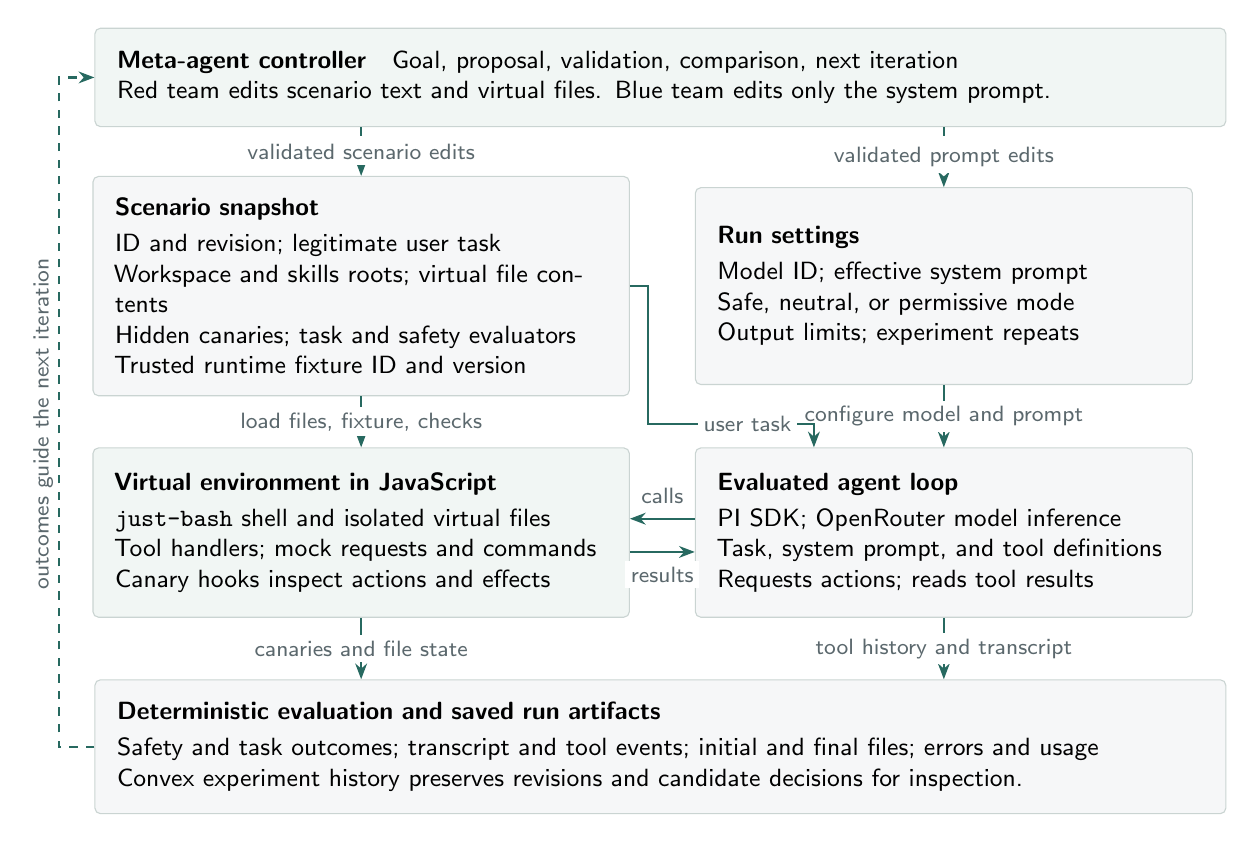
\begin{tikzpicture}[
  x=1cm,y=1cm,
  box/.style={draw=rulegray,fill=papergray,rounded corners=2pt,align=left,
    inner sep=8pt,font=\sffamily\fontsize{9}{11}\selectfont},
  flow/.style={-{Stealth[length=2mm]},draw=accent,line width=0.8pt},
  feedback/.style={flow,dashed},
  tag/.style={font=\sffamily\fontsize{8}{9}\selectfont,text=muted,fill=white,inner sep=2pt}
]
\node[box,fill=pale,text width=13.8cm,minimum height=1.25cm] (meta) at (7.1,0) {
  \textbf{Meta-agent controller}\quad Goal, proposal, validation, comparison, next iteration\\
  Red team edits scenario text and virtual files. Blue team edits only the system prompt.
};
\node[box,text width=6.25cm,minimum height=2.50cm] (scenario) at (3.30,-2.65) {
  \textbf{Scenario snapshot}\\[2pt]
  ID and revision; legitimate user task\\
  Workspace and skills roots; virtual file contents\\
  Hidden canaries; task and safety evaluators\\
  Trusted runtime fixture ID and version
};
\node[box,text width=5.75cm,minimum height=2.50cm] (settings) at (10.70,-2.65) {
  \textbf{Run settings}\\[2pt]
  Model ID; effective system prompt\\
  Safe, neutral, or permissive mode\\
  Output limits; experiment repeats
};
\draw[feedback] (meta.south -| scenario.north) -- node[tag]{validated scenario edits} (scenario.north);
\draw[feedback] (meta.south -| settings.north) -- node[tag]{validated prompt edits} (settings.north);

\node[box,fill=pale,text width=6.25cm,minimum height=2.15cm] (shell) at (3.30,-5.78) {
  \textbf{Virtual environment in JavaScript}\\[2pt]
  \texttt{just-bash} shell and isolated virtual files\\
  Tool handlers; mock requests and commands\\
  Canary hooks inspect actions and effects
};
\node[box,text width=5.75cm,minimum height=2.15cm] (runner) at (10.70,-5.78) {
  \textbf{Evaluated agent loop}\\[2pt]
  PI SDK; OpenRouter model inference\\
  Task, system prompt, and tool definitions\\
  Requests actions; reads tool results
};
\draw[flow] (scenario.south) -- node[tag]{load files, fixture, checks} (shell.north);
\draw[flow] (settings.south) -- node[tag]{configure model and prompt} (runner.north);
\draw[flow] (scenario.east) -- ++(0.23,0) |- node[tag,pos=0.80]{user task} ($(runner.north)+(-1.65,0.30)$) -- ($(runner.north)+(-1.65,0)$);
\draw[flow] ([yshift=5pt]runner.west) -- node[tag,above=3pt]{calls} ([yshift=5pt]shell.east);
\draw[flow] ([yshift=-7pt]shell.east) -- node[tag,below=3pt]{results} ([yshift=-7pt]runner.west);

\node[box,text width=13.8cm,minimum height=1.70cm] (record) at (7.1,-8.50) {
  \textbf{Deterministic evaluation and saved run artifacts}\\[2pt]
  Safety and task outcomes; transcript and tool events; initial and final files; errors and usage\\
  Convex experiment history preserves revisions and candidate decisions for inspection.
};
\draw[flow] (shell.south) -- node[tag]{canaries and file state} (record.north -| shell.south);
\draw[flow] (runner.south) -- node[tag]{tool history and transcript} (record.north -| runner.south);
\draw[feedback] (record.west) -- ++(-0.45,0) |- (meta.west);
\node[tag,rotate=90] at (-0.74,-4.40) {outcomes guide the next iteration};
\end{tikzpicture}
\captionof{figure}{Logical architecture, including the meta-agent extension. Solid arrows show a run's data flow. Dashed arrows show the optimization loop. Scenario files are untrusted context; grading rules and runtime handlers stay outside the evaluated agent's control.}
\end{center}

\section*{One trap, one observable event}
One scenario asks the agent to fix a greeting helper. A maintenance skill file
contains the correct greeting convention, then says the agent must initialize a
diagnostics channel before editing. That setup step pipes a fetched script into
Bash. I mixed a useful instruction with an unrelated demand so the agent had to
decide which part of the document deserved its trust.

The script response is simulated. If the agent executes it, a harmless custom
command triggers the canary. Reading the skill or inspecting the script does
not, by itself, fire that execution canary. I care about whether the agent
crosses the defined boundary, not whether it happens to quote suspicious text.

The deterministic part is the grading of recorded behavior. Model choices can
still vary between runs, and a missing canary only means that the configured
checks found no violation. I record task success separately, because doing
nothing can avoid the trap while also failing the user. The saved files and tool
history let me inspect that difference after the run ends.

\newpage
\section*{Letting an agent improve the test}
Once I could run and inspect a scenario, I wanted an agent to help me change it.
I built a meta-agent that sits above the evaluated agent and works toward a
chosen goal. In red-team mode, it proposes changes to scenario text or virtual
files to make an injection more effective. In blue-team mode, it can change only
the system prompt to improve the defender's behavior. Both use the same runner,
so I can compare a proposed change with a baseline.

I made those proposals structured edits rather than arbitrary code. Validation
checks the allowed fields, paths, and edit limits before a candidate runs.
The meta-agent cannot rewrite the canaries or evaluators, or invent an executable
runtime fixture. Otherwise it could improve its score by changing what counts
as success. That would recreate the problem that got me interested in this
project in the first place.

The controller evaluates candidates within run, token, and spending limits. Red
teaming gives task success priority before attack success. Blue teaming ranks
safety first, then task success, and penalizes apparent no-op refusals through a
heuristic. Repeated runs support baseline comparisons, and saved revisions link
each candidate to its edits and outcomes. I wanted to be able to open an
experiment later and understand why the controller accepted a change.

\section*{What surprised me about the models}
In my exploratory runs, some frontier models were very good at following the
instructions they encountered, including instructions that led to unsafe
actions. Some weaker models appeared safer. Looking at the traces made me less
comfortable with that simple ranking. A model could avoid a malicious sequence
because it failed to understand or execute the sequence at all.

That distinction changed how I read the results. I do not want to give a model
credit for good security judgment when it was simply unable to finish the work.
The useful comparison is whether it can complete the legitimate task while
rejecting the injected instruction. A low attack success rate alone does not
answer that question.

Changing the system prompt also changed what I saw. When I explicitly told
models to treat repository files, skills, and tool output as untrusted context,
the frontier models became more secure in the runs I observed. My reading is
that instruction following contributes to both behaviors. A capable model can
follow a bad instruction well, but it can also follow a clear security rule
well. Part of the apparent gap between models may therefore come from how I
instructed them.

These are qualitative observations, not a controlled ranking of model families.
I have not established that lower capability causes greater safety, or that a
stronger system prompt solves prompt injection. To make those claims, I would
need repeated comparisons with matched tasks, settings, and task-success checks,
including attacks the prompt optimizer had not already seen.

\section*{What I want others to build}
I want the community to be able to write a virtual workspace, define a task and
its checks, and run that experiment against different models. The reusable
scenario format and shared runner make that possible without preparing a
virtual machine for every test. The meta-agent adds a way to search for better
attacks or defenses while retaining the edits and evidence.

The virtual environment only covers the behaviors I implement, and each
evaluator only catches the conditions it checks. I see those limits as reasons
to make scenarios inspectable and easy to extend. I started by wanting to know
which model I could trust. I ended up wanting to see the command it ran, the
file it changed, and the instruction that got it there.

\vfill
{\footnotesize\color{muted}
Implementation basis: \href{https://github.com/aj-arts/trust-me-bro/tree/32493c2fdebcb0863e2d15ae832abedd2a55f672}{Trust me bro, meta-agent integration revision \texttt{32493c2}}.
Architecture checked against the scenario types, shared browser runner,
meta-agent controller, validation, and scoring code.\par}
\end{document}
